\section{Performance Evaluation}\label{sec:evaluation}

This section presents a comprehensive performance evaluation of \iblock{},
focusing on execution time, memory usage, and performance scaling. We analyze
scaling trends to assess how \iblock{} adapts to larger networks and
transaction volumes and outline potential methods for reducing simulation
time and memory consumption in large network simulations.

\subsection{Execution Time and Memory
Usage}\label{subsec:execution-time-memory-usage}

To establish a baseline understanding of \iblock{}'s performance, execution
time and memory consumption were measured for a scenario with 80 nodes,
including 15 miners. In this scenario, each node generates a transaction
approximately every 30 seconds, with statistics recording enabled in default
\textit{recording mode}. This configuration prioritizes essential statistics,
typically aggregating key data and limiting vector tracking.

The configuration for this scenario, defined in \texttt{simulations/perf.ini}
and labeled as ``BigNetPerformance'', was executed for a simulated period of 10
days. A Bash script sampled the process periodically, recording execution time
and memory usage.

\figref{fig:bnp-memory-usage} illustrates the memory usage (resident set size)
over time as a percentage of the total real-world execution time. Memory usage
reached a peak of approximately \(13.18\) GB, with an increase that is
sublinear in relation to the simulation duration.

\begin{figure}[tbhp]
	\centering
	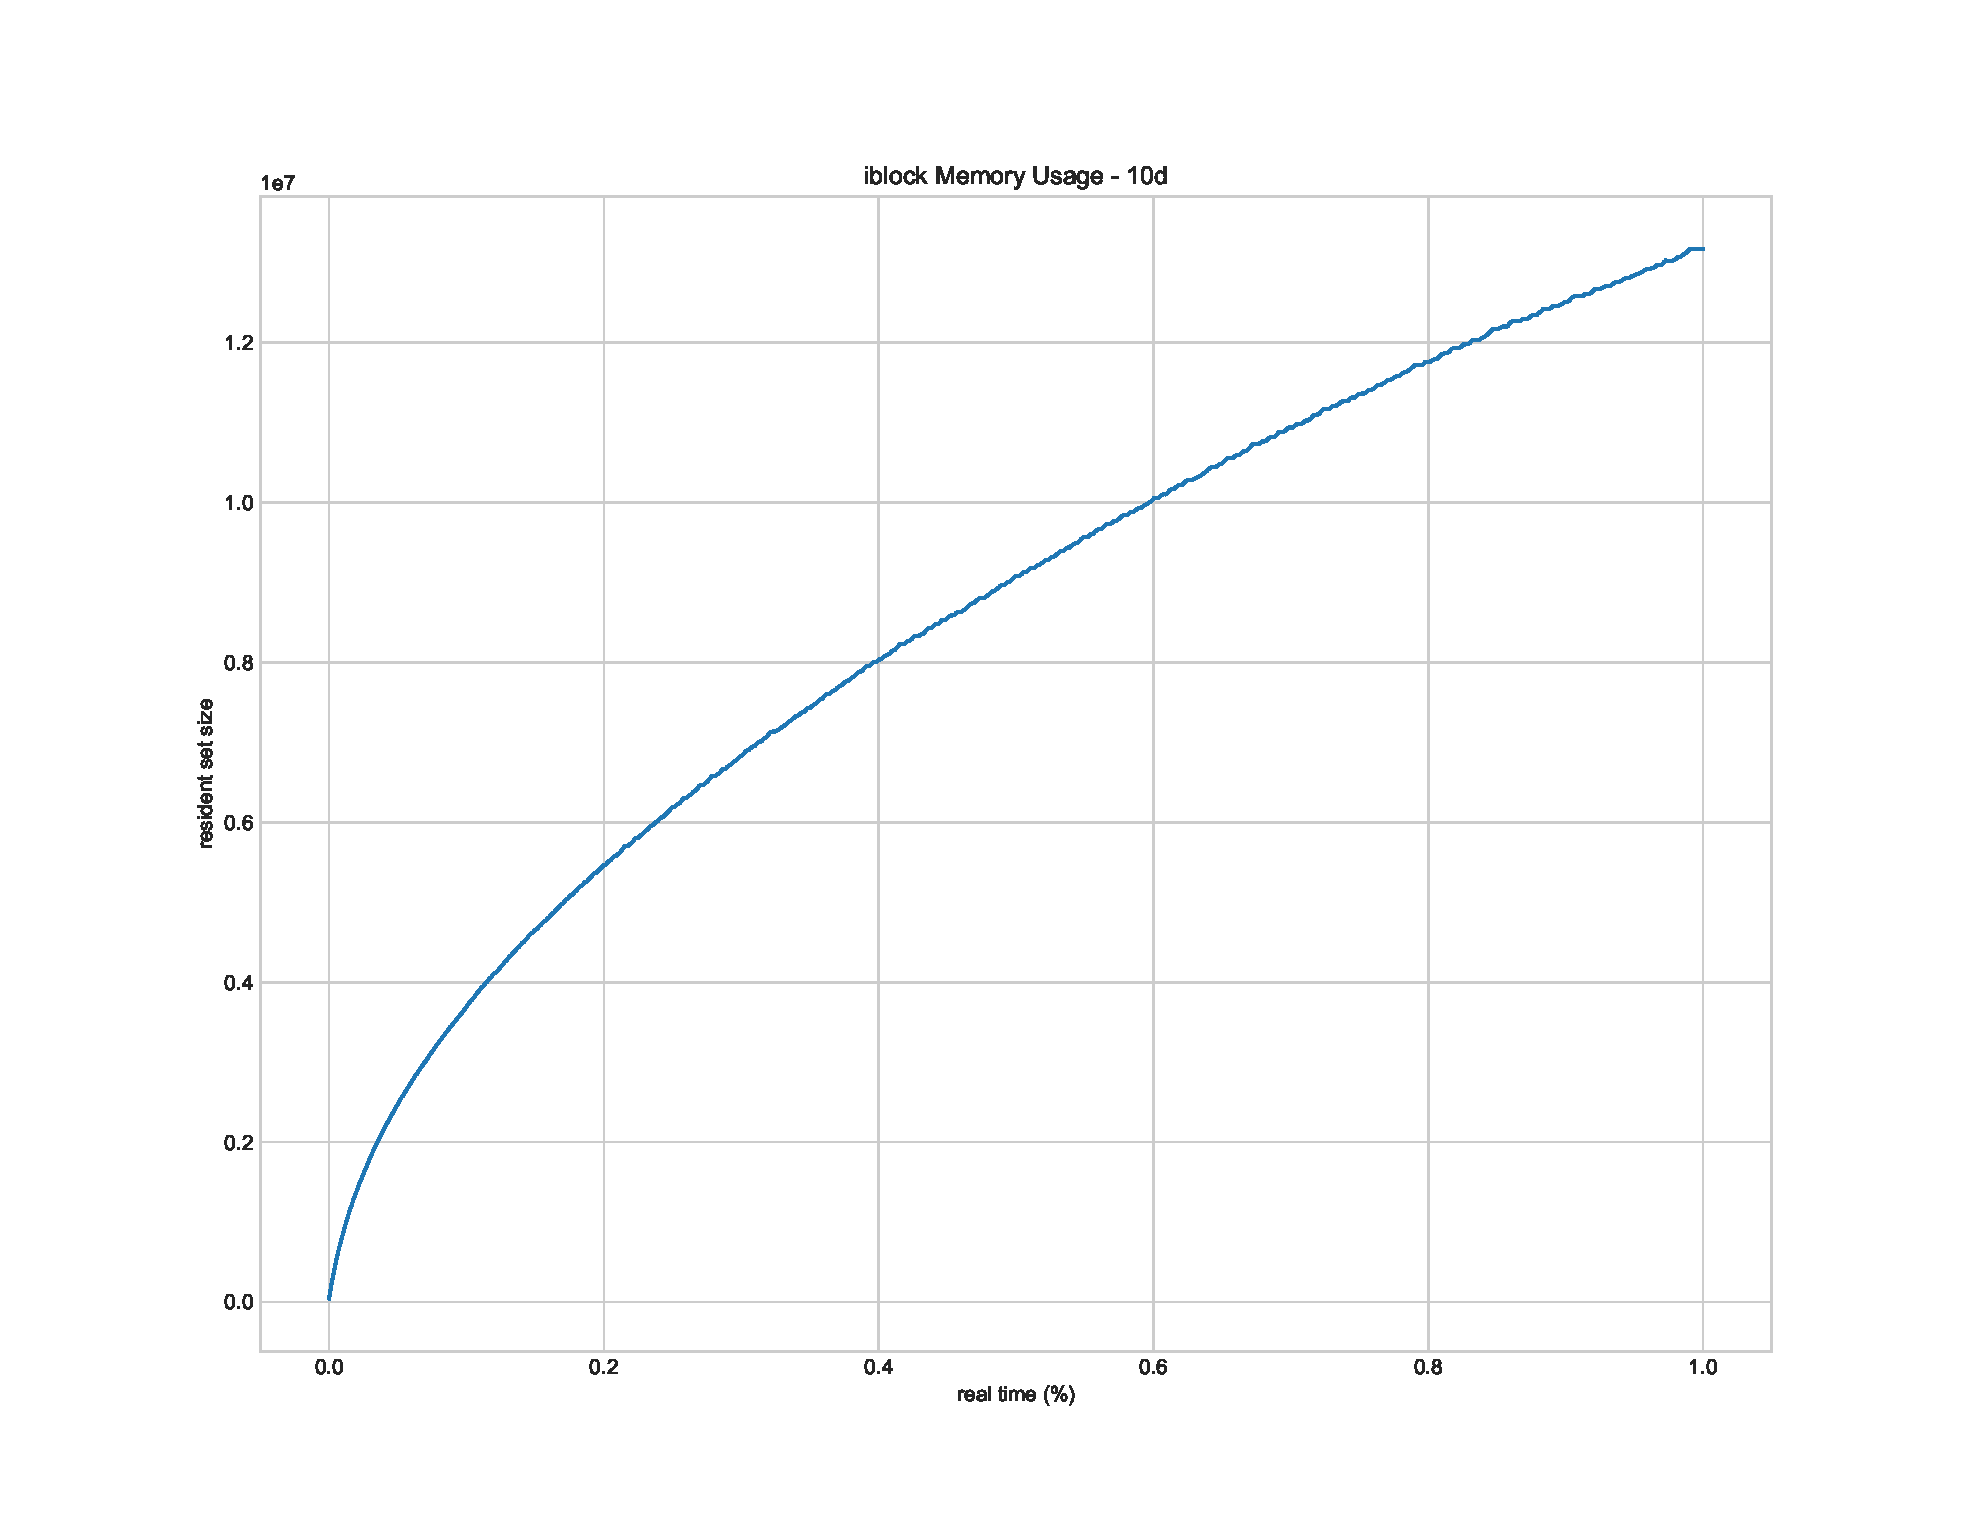
\includegraphics[width=\textwidth,trim={3.05cm 1.85cm 3.3cm
	2.5cm},clip]{bignet-mem-usage}
	\caption{Memory usage of \iblock{} over time, for the
	``BigNetPerformance'' configuration.}\label{fig:bnp-memory-usage}
\end{figure}

Table \ref{tab:bnp-performance} summarizes the simulation's execution time and
memory usage after each simulated day, along with a
simulation-time-to-real-time ratio as an indicator of simulation speed over
time. Additionally, \figref{fig:bnp-execution-time} shows the real execution
time required to simulate each 12-hour segment of the scenario.

\begin{table}[tbhp]
	\centering
	\begin{tabular}{|c|c|c|c|}
		\toprule
		Day & Execution Time & This Day Exec\@. Time (\(\Delta\)) & Simulation Speed (\(\Delta\)) \\
		& & & \textit{\small simsec/sec} \\
		\midrule
		1\textsuperscript{st} & 1m\,40s & 1m\,40s & \(864.0\) \\[6pt]
		2\textsuperscript{nd} & 4m\,57s & 3m\,17s (+1m\,37s) & \(438.58\) (\(-425.42\)) \\[6pt]
		3\textsuperscript{rd} & 9m\,52s & 4m\,55s (+1m\,38s) & \(292.88\) (\(-145.7\)) \\[6pt]
		4\textsuperscript{th} & 16m\,23s & 6m\,31s (+1m\,36s) & \(220.97\) (\(-71.91\)) \\[6pt]
		5\textsuperscript{th} & 24m\,27s & 8m\,4s (+1m\,33s) & \(178.51\) (\(-42.46\)) \\[6pt]
		6\textsuperscript{th} & 33m\,50s & 9m\,23s (+1m\,19s) & \(153.46\) (\(-25.05\)) \\[6pt]
		7\textsuperscript{th} & 44m\,38s & 10m\,48s (+1m\,25s) & \(133.33\) (\(-20.13\)) \\[6pt]
		8\textsuperscript{th} & 56m\,36s & 11m\,58s (+1m\,10s) & \(120.33\) (\(-13\)) \\[6pt]
		9\textsuperscript{th} & 1h\,10m\,11s & 13m\,35s (+1m\,37s) & \(106.01\) (\(-14.32\)) \\[6pt]
		10\textsuperscript{th} & 1h\,25m\,38s & 15m\,27s (+1m\,52s) & \(93.20\) (\(-12.81\)) \\
		\bottomrule
	\end{tabular}
	\caption{Time needed to simulate each day and simulation speed.}\label{tab:bnp-performance}
\end{table}

\begin{figure}[tbhp]
	\centering
	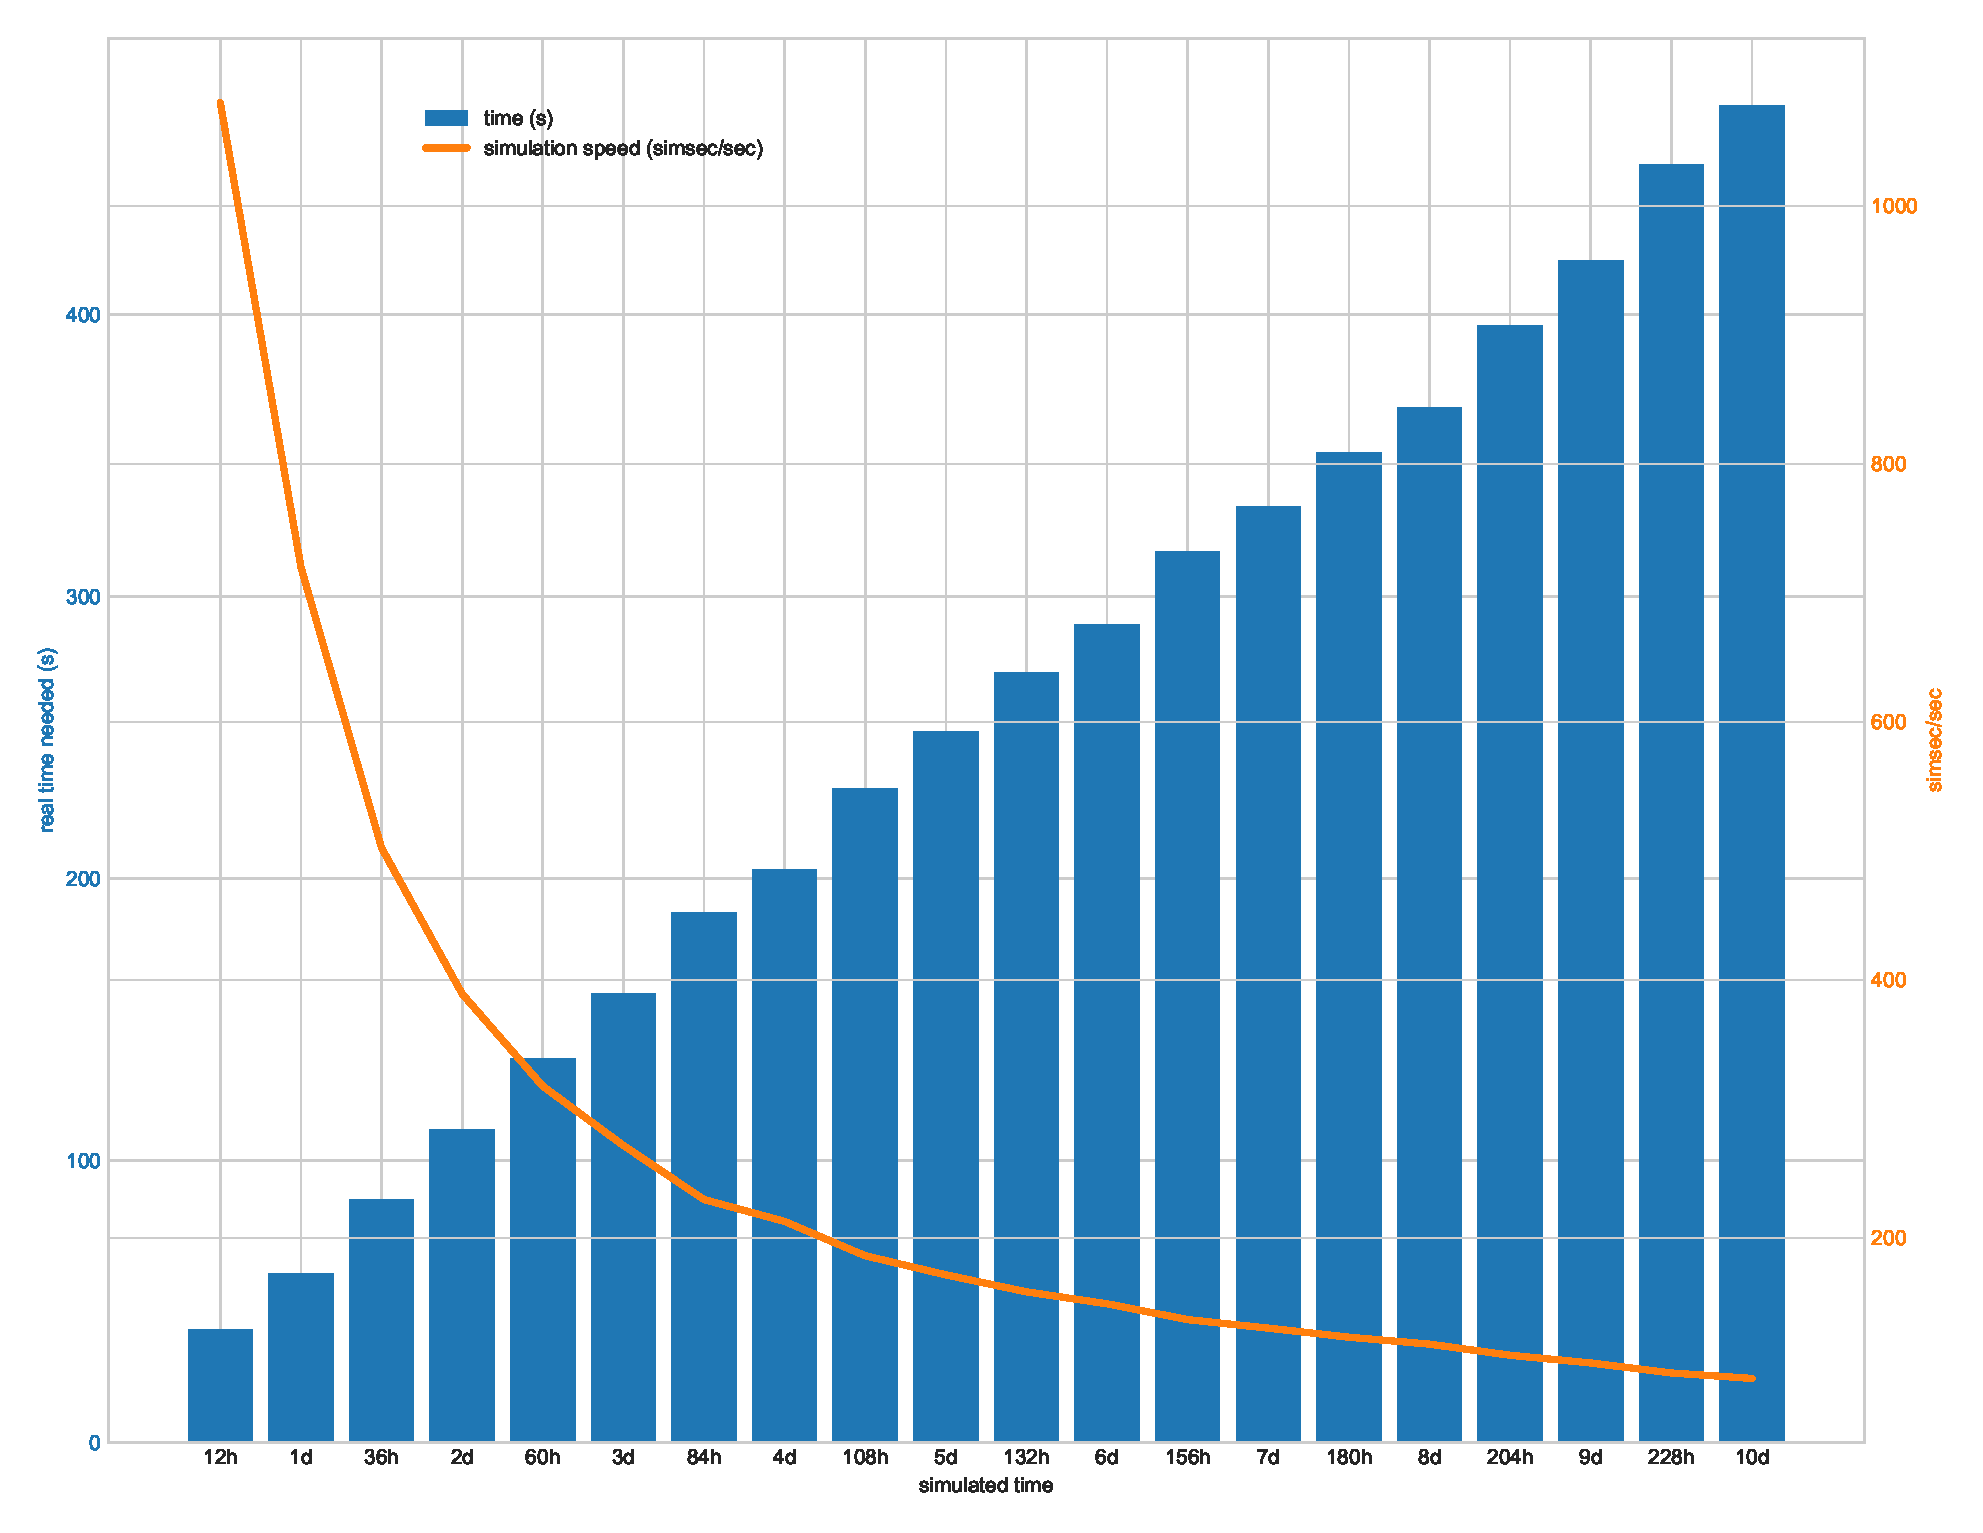
\includegraphics[width=\textwidth]{bignet-exec-time}
	\caption{Execution time for each 12-hour segment (histogram) and
	simulation speed in terms of simsec/sec
	(line).}\label{fig:bnp-execution-time}
\end{figure}

Execution time for each 12-hour segment increased by about 20--30 seconds
compared to the previous segment, indicating a linear trend. This increase is
expected, as each new transaction generation requires iterating over an
expanded set of UTXOs in each node's wallet to verify available funds. The
corresponding memory usage rise can be similarly attributed to the growing
number of UTXOs stored.

\subsection{Performance Scaling}\label{subsec:performance-scaling}

In this section, the scalability of \iblock{} is evaluated by varying network
size and transaction rates. This allows us to gauge \iblock{}'s execution time
and memory consumption under different levels of network complexity and
transaction intensity.

\subsubsection{Scaling with the Number of Nodes}\label{subsubsec:scaling-nodes}

\figref{fig:scaling-nodes} depicts how execution time and maximum memory usage
change as the number of nodes in the network is increased in increments of 10,
from 10 up to 50 nodes. For consistency, miners were set to comprise
\(\frac{1}{5}\) of the total node count, and the network was configured to
produce a constant rate of three transactions per second.

\begin{figure}[tbhp]
	\centering
	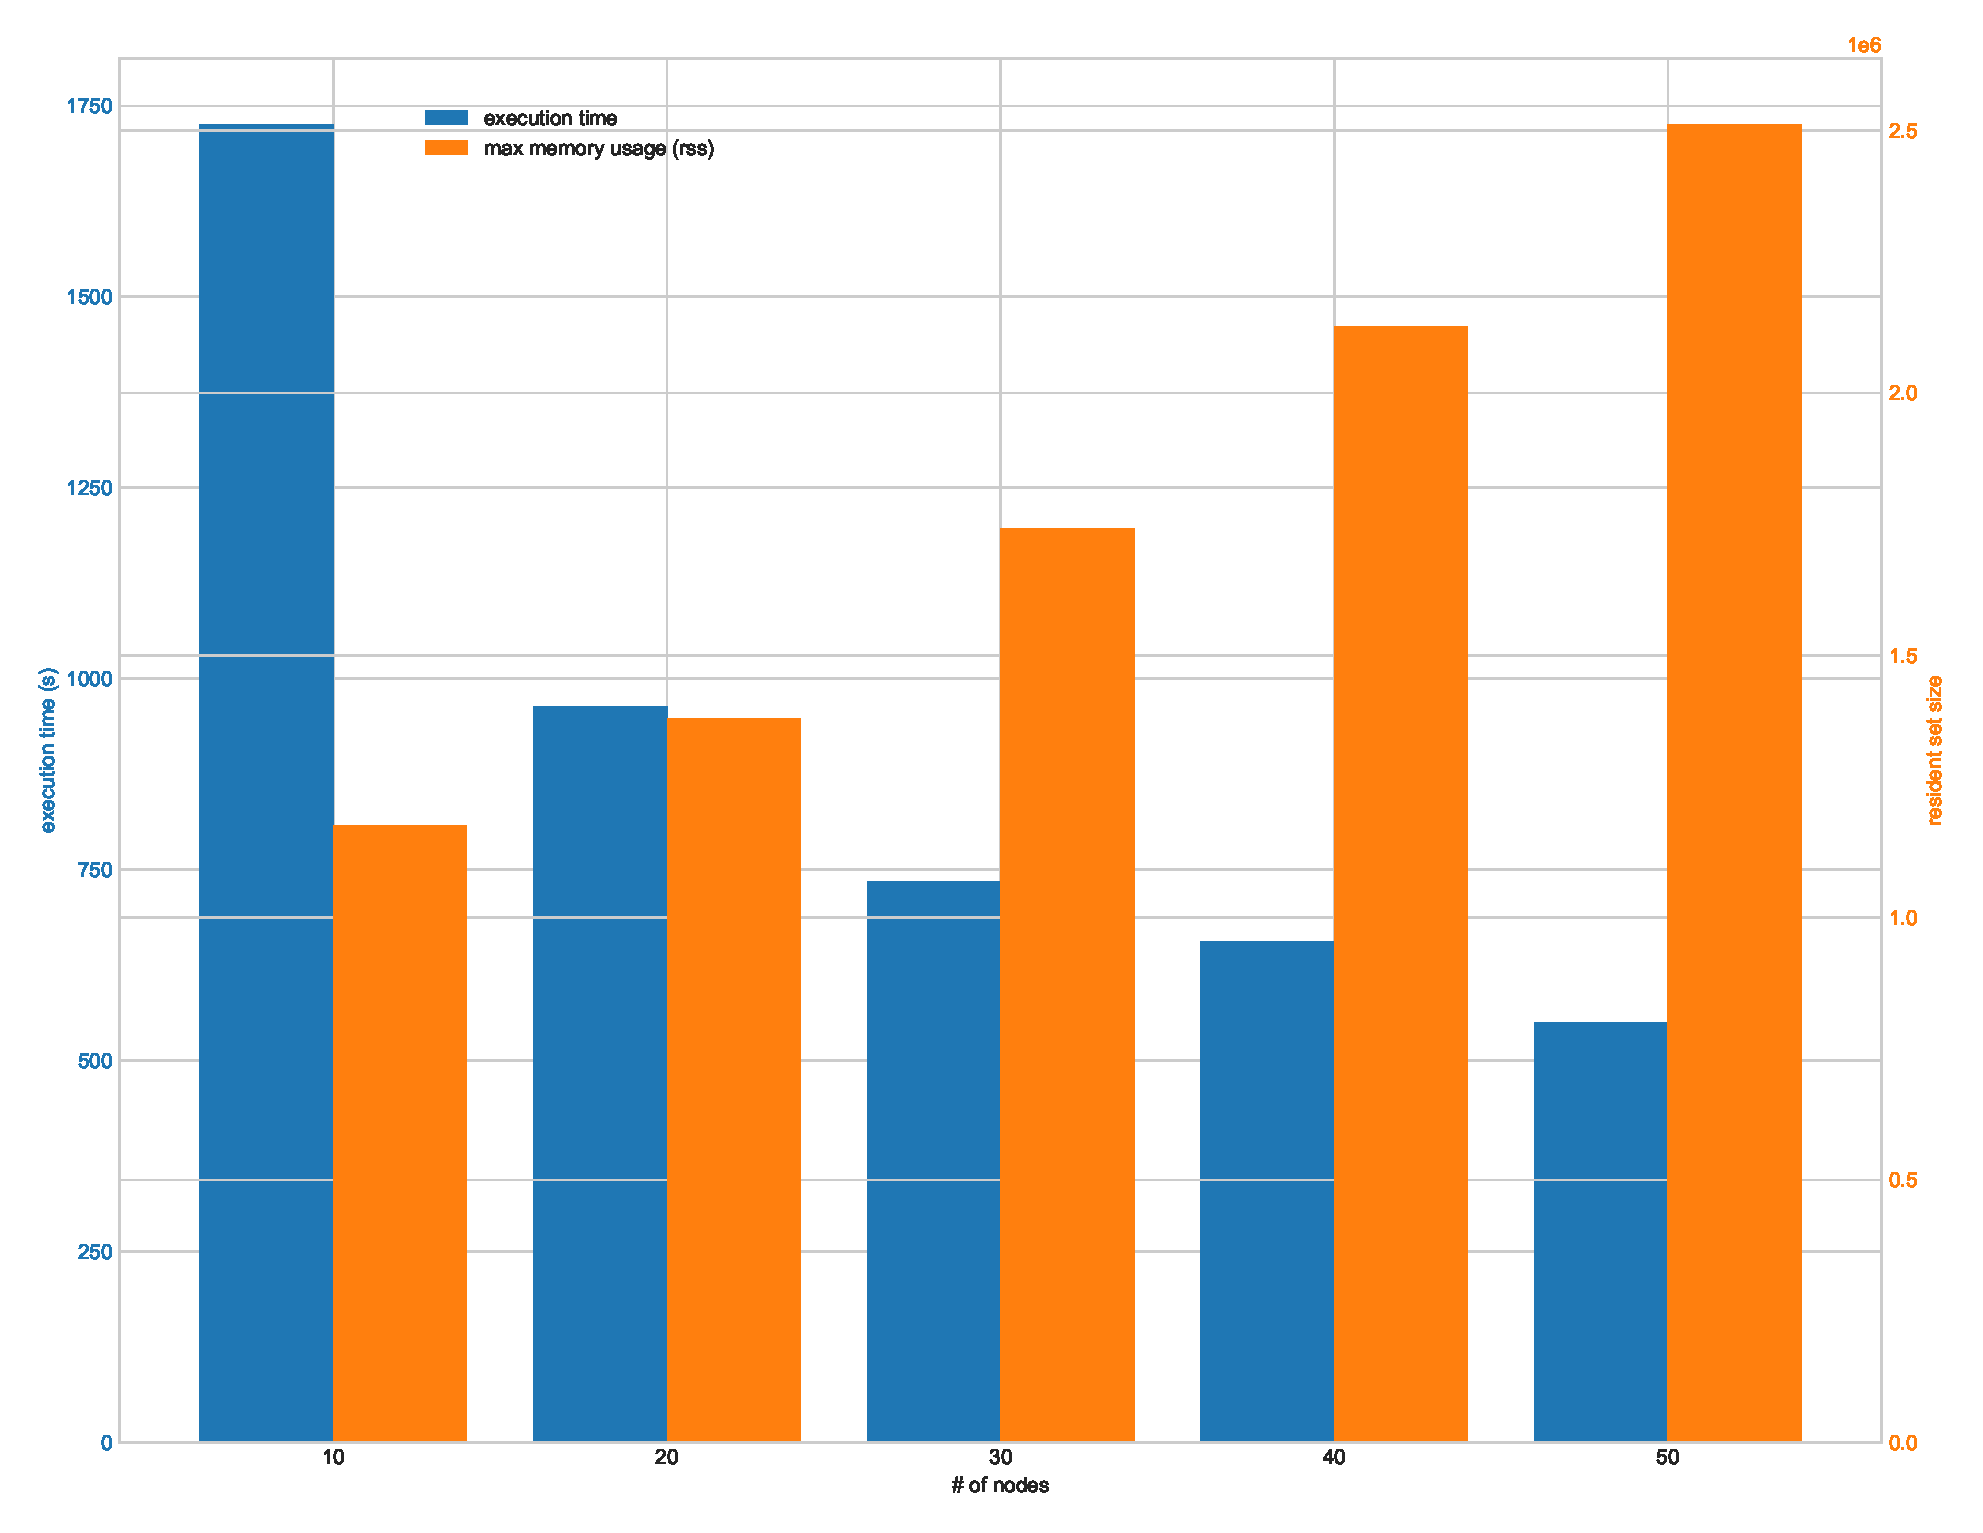
\includegraphics[width=\textwidth]{scaling-nodes-perf}
	\caption{Total execution time (blue) and maximum memory resident set
	size (orange) of \iblock{} while varying the number of nodes in the
	network.}\label{fig:scaling-nodes}
\end{figure}

The configuration for this experiment, ``ScalingNodesPerformance'', is located
in \texttt{simulations/perf.ini}, with each simulation running for three
simulated days.

Interestingly, the execution time decreases as the node count increases. This
counterintuitive outcome results from the constant transaction rate: as nodes
increase, the UTXOs become more distributed among them, reducing each node's
average UTXO count. Consequently, each node requires less time to locate
available funds for transactions. This effect is particularly noticeable
because transaction generation, occurring continuously, is far more frequent
than block generation, which happens every 10 minutes.

In contrast, memory usage grows as the node count increases, as each node must
maintain its own version of the mempool. More nodes result in more different
mempools, thus increasing overall memory consumption.

\subsubsection{Scaling with the Transaction Rate}\label{subsubsec:scaling-tx}

\figref{fig:scaling-tx} shows how execution time and peak memory usage change
as the network transaction rate increases from \(0.5\) to \(4.0\) transactions
per second in \(0.5\) increments. For this simulation, a network of 30 nodes
was used, with six miners.

\begin{figure}[tbhp]
	\centering
	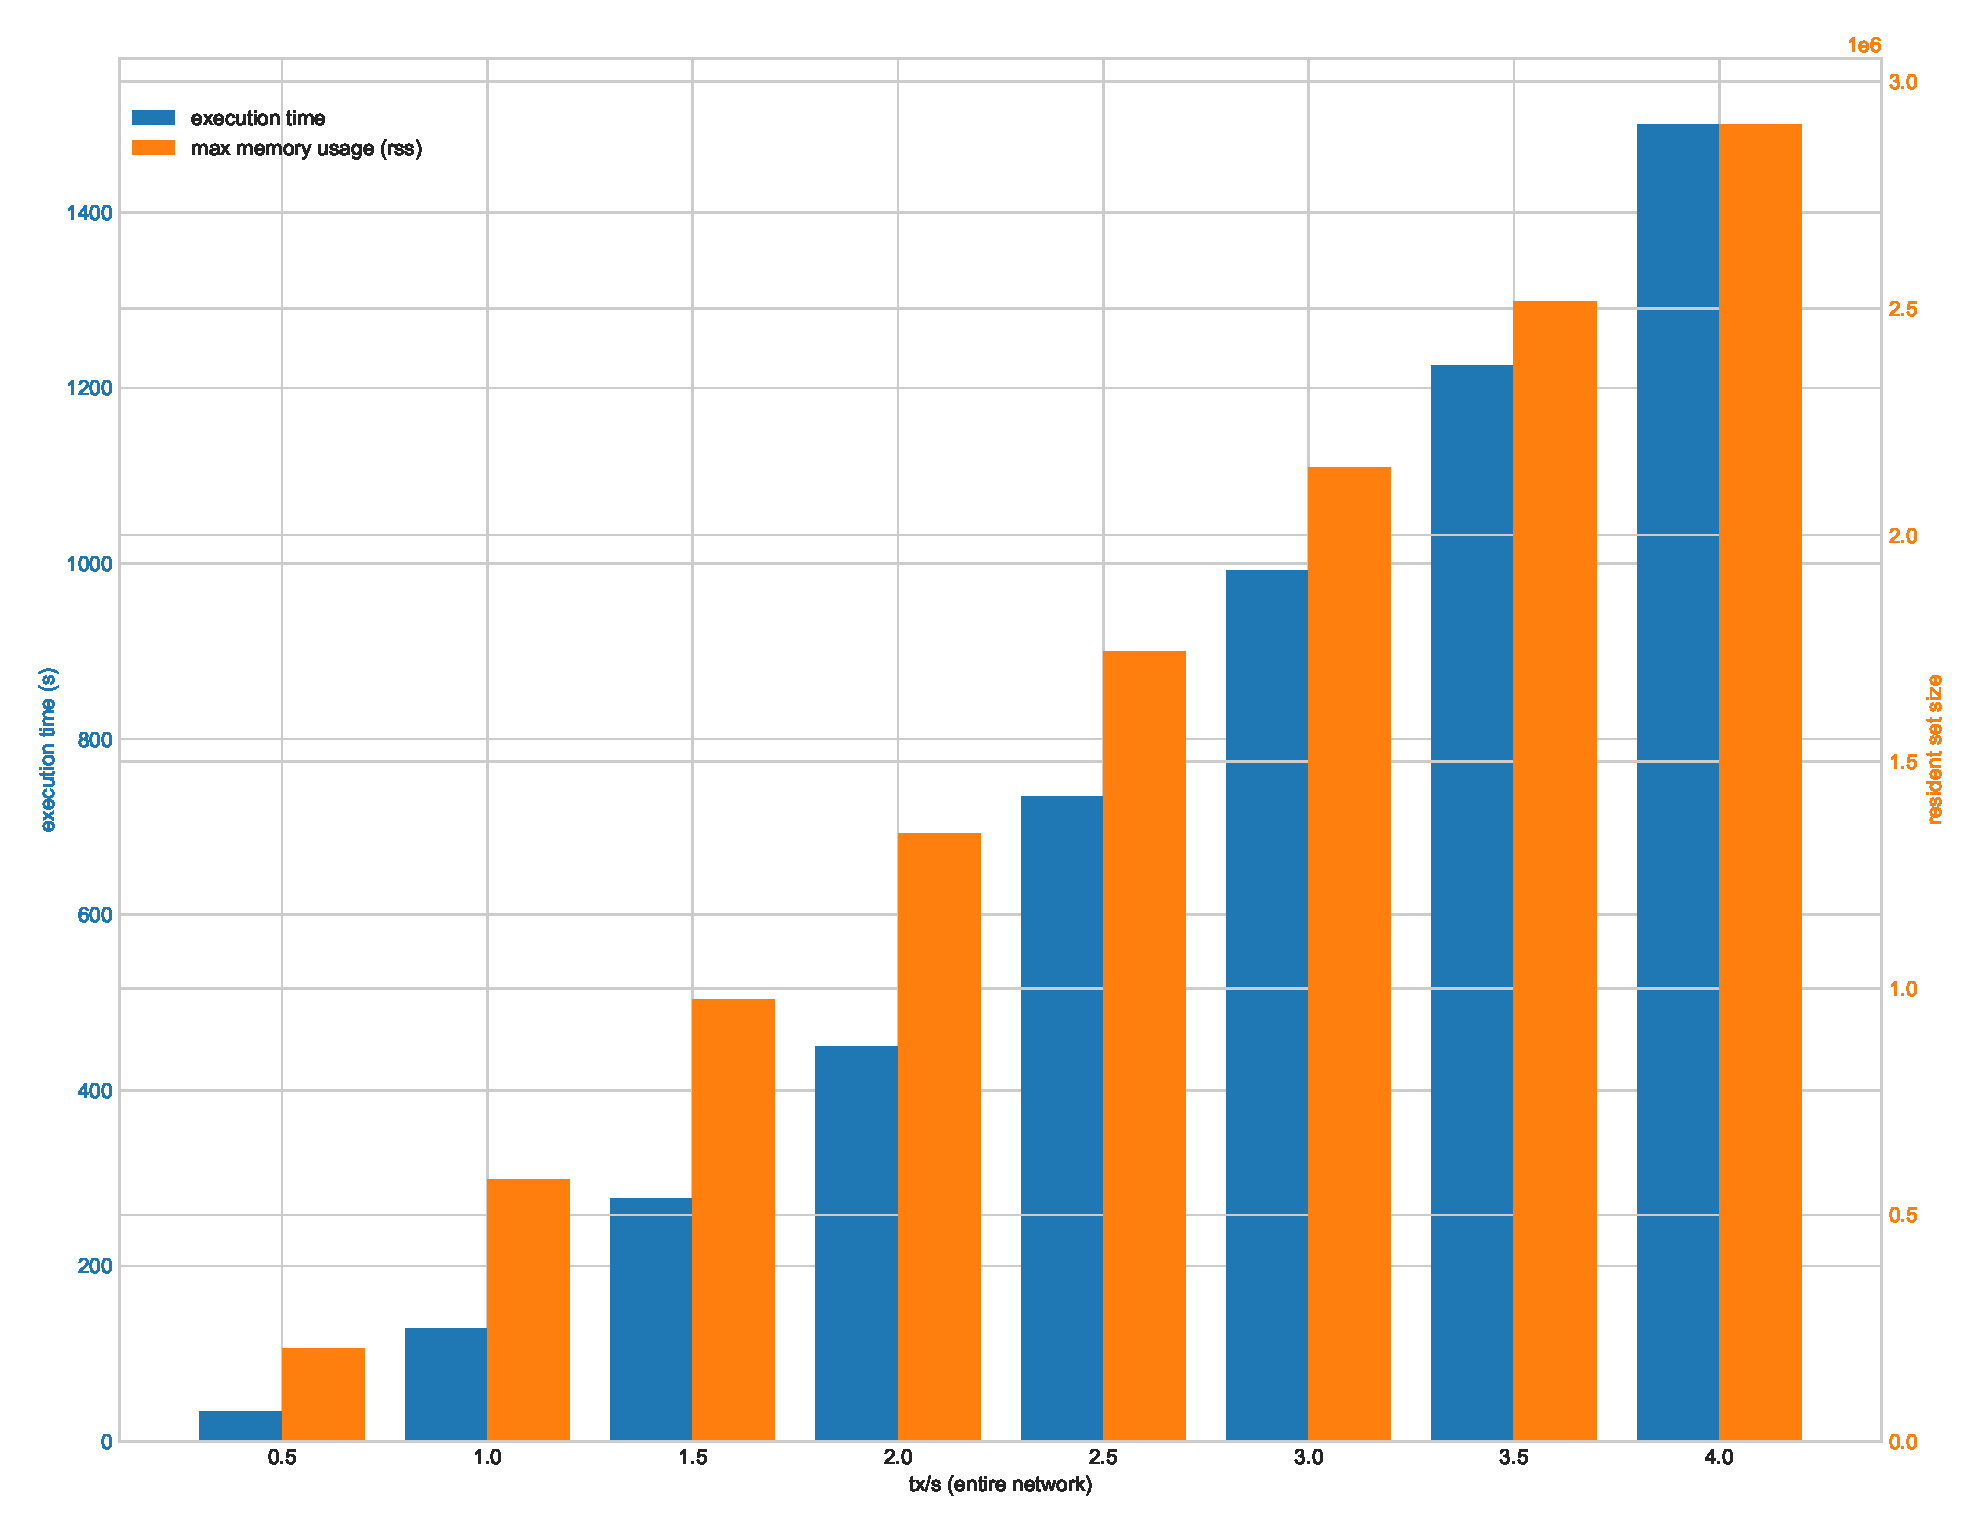
\includegraphics[width=\textwidth]{scaling-txgen-perf}
	\caption{Total execution time (blue) and maximum memory resident set
	size (orange) of \iblock{} while varying the number of transactions per
	second generated by the network.}\label{fig:scaling-tx}
\end{figure}

The configuration for this experiment, ``ScalingTxGenPerformance'', is also
located in \texttt{simulations/perf.ini}, with each simulation running for
three simulated days.

As the transaction rate increases, both execution time and memory usage rise
correspondingly. Execution time increases due to the higher number of
transactions the network must process (transaction generation events are more
frequent). Additionally, each node's UTXO set expands, making fund
verification more time-consuming. Memory usage similarly increases, as each
node must handle a larger mempool and UTXO set.

\subsubsection{Scaling Both Network Size and Transaction
Rate}\label{subsubsec:scaling-both}

\figref{fig:scaling-both} illustrates how execution time and memory usage
changes as both the number of nodes and the \emph{global} transaction rate
increase. The transaction rate \emph{per node} is kept constant at 1
transaction every 12 seconds. As above, each simulation has been run for three
simulated days. Table~\ref{tab:scaling-both} provides the exact configuration
for each run.

\begin{table}[tbhp]
	\centering
	\begin{tabular}{|c|c|c|c|c|}
		\toprule
		Run \# & \# of Nodes & \# of Miners & Tx interval (per node) & Tx/s (global) \\
		\midrule
		1 & 10 & 2 & 12s & \(0.8333\) tx/s \\\midrule
		2 & 20 & 4 & 12s & \(1.6667\) tx/s \\\midrule
		3 & 30 & 6 & 12s & \(2.5\) tx/s \\\midrule
		4 & 40 & 8 & 12s & \(3.3333\) tx/s \\\midrule
		5 & 50 & 10 & 12s & \(4.1667\) tx/s \\
		\bottomrule
	\end{tabular}
	\caption{Configuration for the ``ScalingBothPerformance''
	experiment.}\label{tab:scaling-both}
\end{table}

\begin{figure}[tbhp]
	\centering
	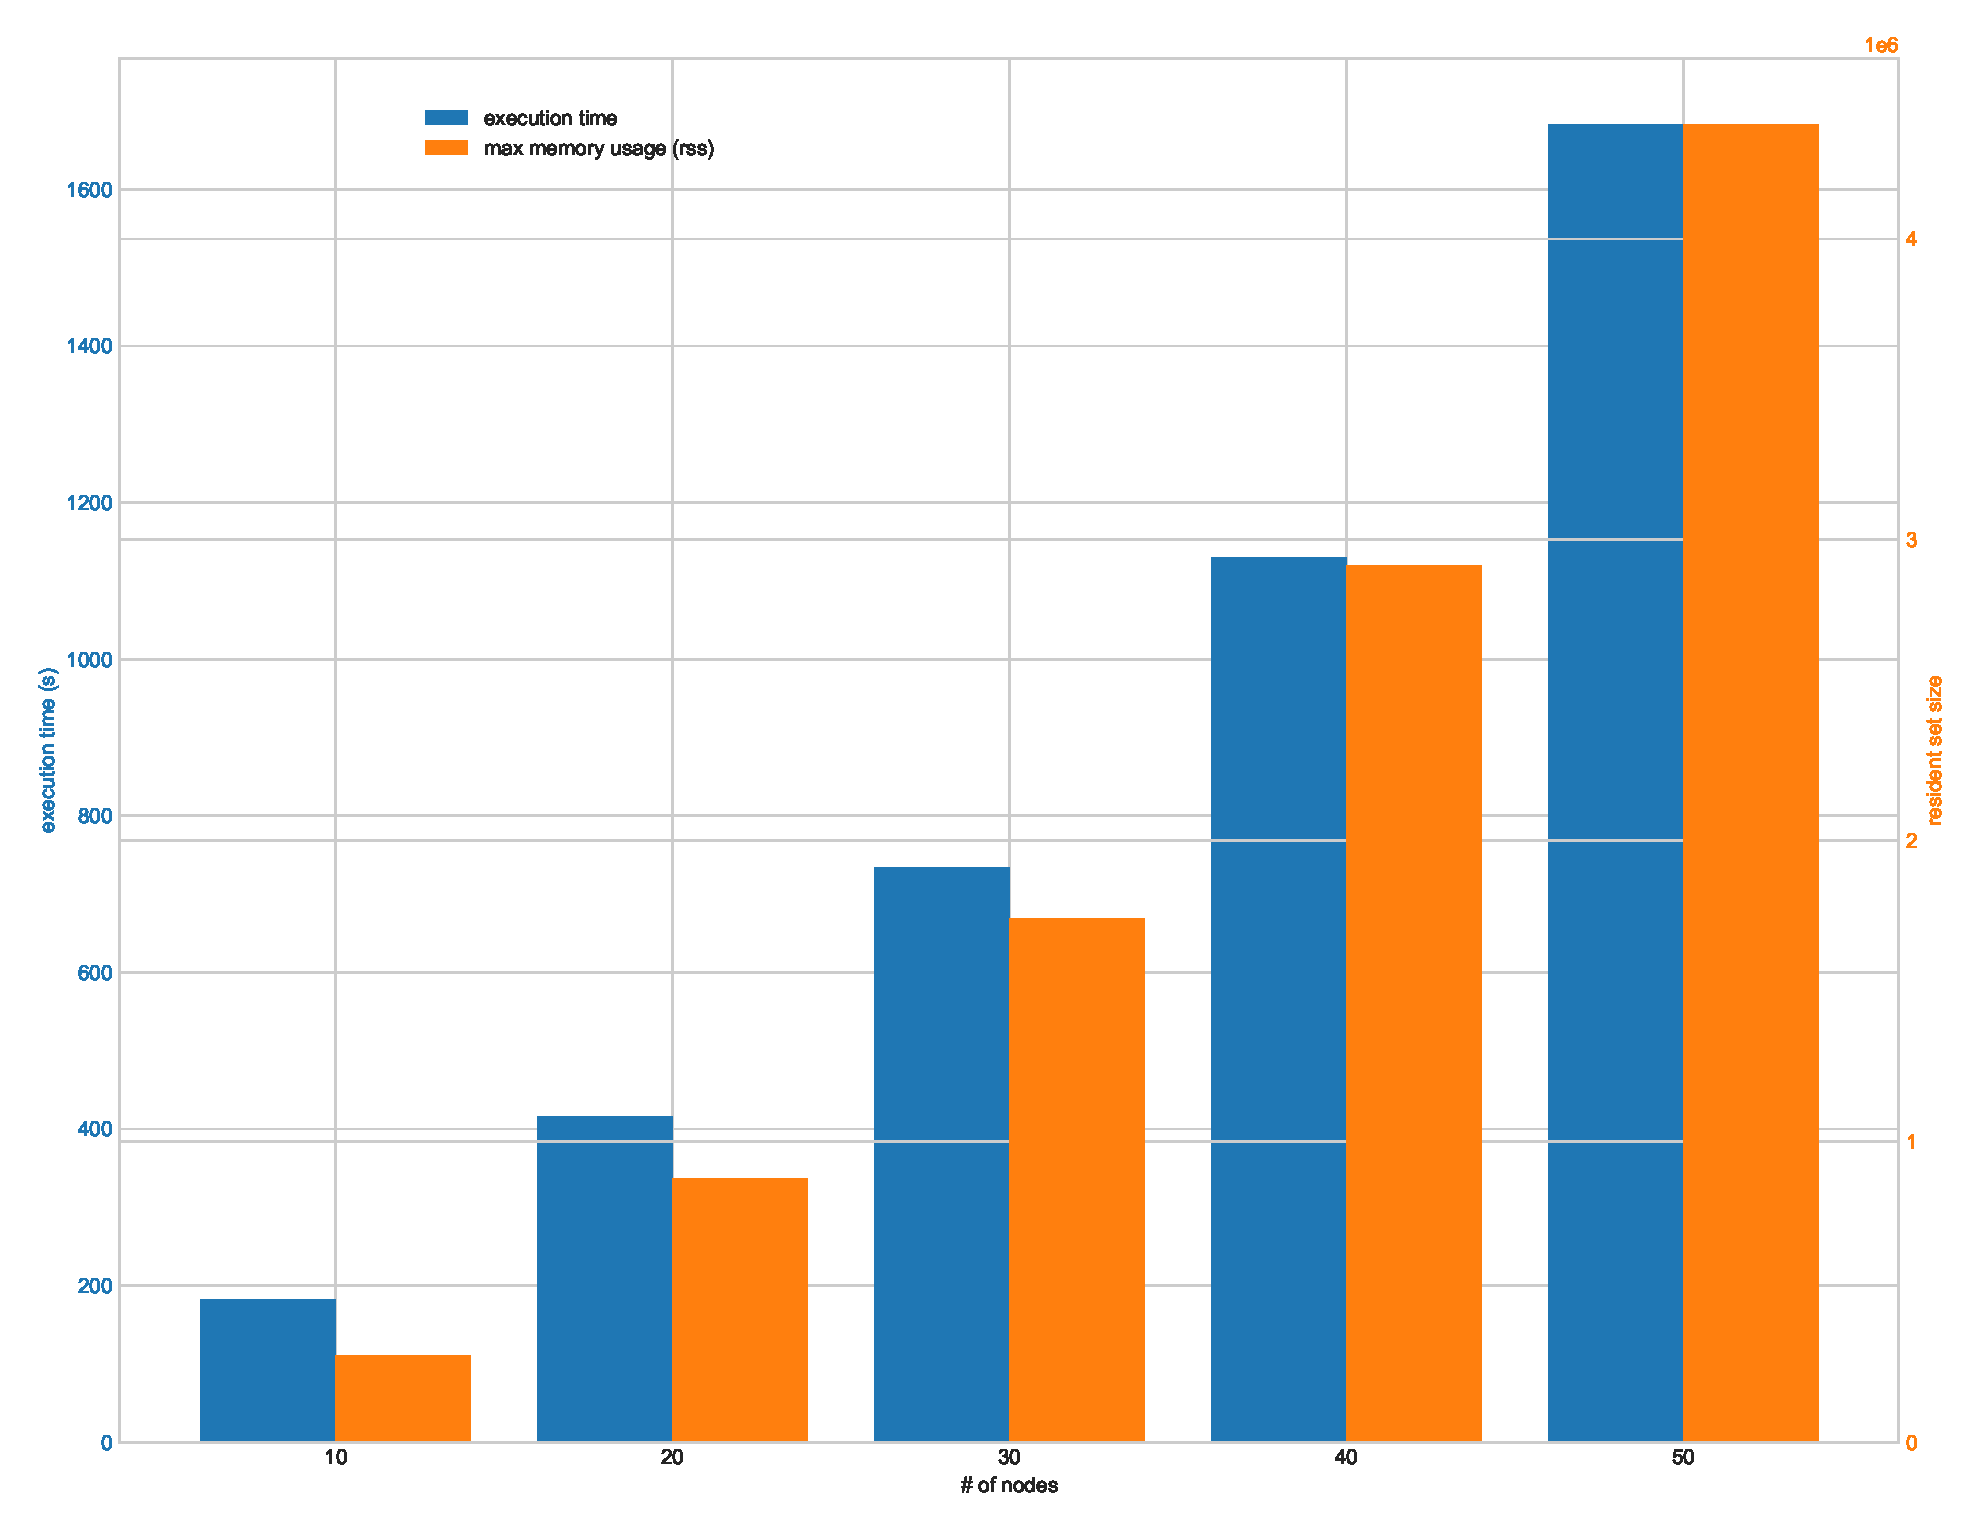
\includegraphics[width=0.9\textwidth]{scaling-both-perf}
	\caption{Total execution time (blue) and maximum memory resident set
	size (orange) of \iblock{} while varying the number of nodes and
	keeping a constant transaction rate per node (increasing global
	transaction rate).}\label{fig:scaling-both}
\end{figure}

Results show that both execution time and memory usage increase as the network
size and global transaction rate grow. The increase in execution time is mainly
determined by the higher number of transactions generated by the network. In
this case, there is no more the effect of the UTXO set distribution among the
nodes as in \figref{fig:scaling-nodes}, as the transaction rate per node is
kept constant. Larger mempools and higher number of different mempools
contribute to the memory usage growth.

\subsection{Conclusions}\label{subsec:performance-conclusions}

The results above demonstrate that \iblock{} is capable of simulating networks
with tens of nodes (or some hundreds of nodes, if enough memory is provided)
and moderate transaction rates (similar to Bitcoin's throughput of
approximately \(3.3\)--7 transactions per second). Memory usage currently poses
the primary constraint, though increased memory availability can support larger
networks.

To simulate thousands of nodes and higher transaction rates, network scaling
techniques can be employed. For example, instead of simulating a network with
\(1000\) nodes (100 miners) at 10 transactions per second, one could simulate a
smaller network with 100 nodes (10 miners) generating transactions at the same
rate but producing smaller blocks (e.g., \(0.1\) MB instead of 1 MB).

While the simulation results require post-simulation scaling adjustments to
align with real-world network conditions, this approach preserves network
behavior and is a commonly used technique in large-scale system simulations.
